
\lfoot{William Matthews}

\section{Introduction}
\subsection{Outline}

In this project a design draft of an ammonia-based Energy Storage System (ESS) is presented.
The plant and wind farm have to power the island of Maui on its own, with no support from other generation units.


\subsection{What is an ESS?}

An Energy Storage System is a means of capturing excess energy in an electrical transmission grid to be used later.
ESSs are seeing an increase in their potential use as many renewables only offer power intermittently. There is an upwards trend in amount of renewables used \cite{intro:growth} meaning a method to supply consumers power all the time is needed.

\subsection{Location, and why implement an ESS?}

In the scenario given, the plant has to power a location with nothing more than an ESS and a wind farm.
The location chosen (after considering various options through a multi-criteria analysis) was the island of Maui, Hawaii.
The primary considerations leading to the choice of this location were:
\begin{description}
        \item[Fuel Imports]{Hawaii is primarily powered by oil \cite{intro:oilimport} which has to be imported by a fuel tanker. Importing oil adds to the carbon footprint of the generation, as well as the cost of the power made. Eliminating the need to import a fuel via tanker should remove some of the cost associated with generation.}
        \item[High Energy Price]{Hawaii has the highest electrical prices in the USA, at \$0.3114 per kWh (residential January 2018)\cite{intro:price}. The Next highest state is Rhode Island at \$0.2224 per kWh (residential January 2018)\cite{intro:price}. Average US electrical prices across the residential sector is \$0.1223 per kWh (January 2018)\cite{intro:price}. As Hawaii has almost triple the prices across the rest of the US, this seems like a good opportunity to penetrate the market with a more cost-effective solution that the consumers will back.
Hawaii's population is high and it continues to grow year-on-year, meaning extra capacity will have to be built in to satisfy consumer's demands for the future. Of course, as technology and time progresses, the population grows more power-hungry.}
        \item[Clean Energy Initiative]{On January 28, 2008, the State of Hawaii and the USDE (US Department of Energy) signed a `Memorandum of Understanding' with the goal to use renewable resources such as wind, sun, ocean, geothermal and bio-energy to supply 70\% or more of Hawaii's energy needs by 2030 to reduce the State's dependence on imported oil.}
        \item[Geography]{Windspeeds in the State of Hawaii are high making this an ideal location for wind power \cite{intro:windspeed}. To supplement this, the U.S. Department of Energy identified Hawaii to have the potential to install 3,000 MW of wind power, capable of generating 12,000 million kWh per year \cite{intro:energy}.
Considering that the entire State used only 9,962 million kWh in 2011, this project seems feasible with efficient processes.}
\end{description}

\subsection{Project Aims}

It is also useful to consider some of the non-obvious project aims that will be tackled in this report:
\begin{description}
        \item[Sustainable]{Sustainability is very important in this plant, as it must be a better alternative to the current oil infrastructure, with the future in mind as well. Sustainability covers environmental and social considerations, which covers everything from reducing resource use, reducing pollution, as well as ensuring social acceptance. Sustainable design was considered for each process unit to maximise the sustainability metrics decided on, while delivering the specified material flow rates required for self-sufficient design. Sustainability is explored in its own section in more depth in this report.}
        \item[Profitable]{For this design to be a viable suggestion of replacing Hawaii's oil infrastructure, it \emph{must} be able to run a profit over the plant's lifetime, otherwise such a plant will not be attractive to investors. This is explored below in the Costing section.}
        \item[Safe]{Running a large chemical plant has a lot of hazards associated with it, and careful consideration of these through HAZOP and risk analysis is required before an implementation of the plant can occur. For instance, the energy storage medium used, ammonia, can cause harm to people should a leak occur, careful planning with HAZOP and risk analysis can aid in making the plant safer and more socially acceptable. Plant safety is explored in its own section below.}
        \item[Satisfies Demand]{For this plant to replace the current infrastructure it must run entirely by itself. The plant must generate and store ammonia, for use in a generation stage to satisfy local demand. The entire process flow is explored through through component design sections below. }
\end{description}

\subsection{Plant Structure}

The plant structure is setup as in Figure \ref{fig:plantglobaldiagram} and sub-divided into sections that are discussed below in detail.
The most complex parts of the components are explored to see how the objective of supplying power to Maui can be achieved solely using wind power and storing energy in ammonia.

\begin{figure}[p]
        \centering
        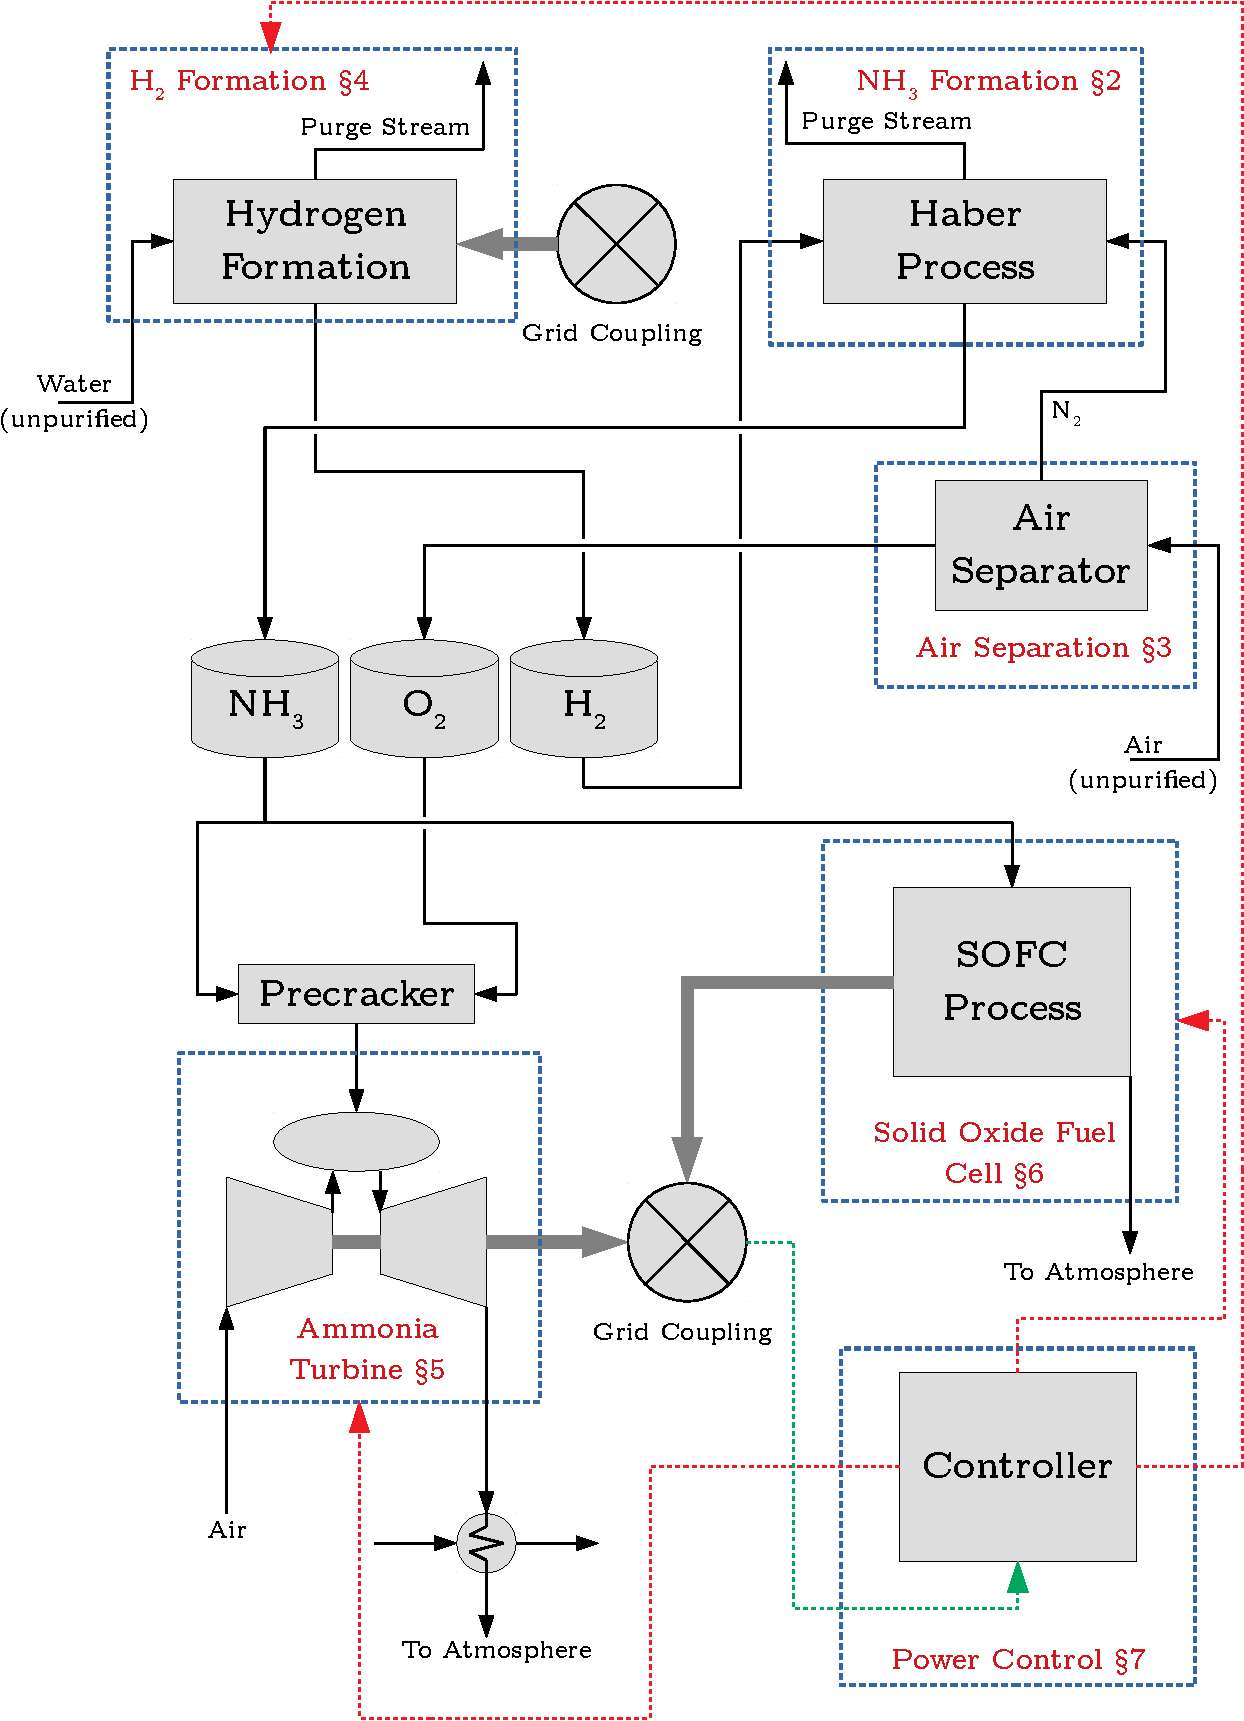
\includegraphics[scale=0.7]{plantdiagram.pdf}
        \caption{Diagram Showing Component Interconnections}
        \label{fig:plantglobaldiagram}
\end{figure}

\bibliographystyle{unsrt}
\bibliography{./intro/introbib}
%\bibliography{introbib}